\newcommand{\noteOnBitcoinNaming}[0]{\footnote{
    From now till the end of the document, we will use the word Bitcoin capitalized to identify the protocol,
    and the word bitcoin not capitalized to identify the currency
    }
}

\chapter{Bitcoin}
\label{chap:bitcoin}

\section{Introduction}

Bitcoin is a digital currency that uses \emph{blockchain} technology to track
and verify transactions. It was created in 2009 by an unknown individual or
group using the pseudonym \emph{Satoshi Nakamoto}.
Bitcoin is decentralized, meaning that it is not controlled by any government
or institution. Instead, it relies on a network of computers around the world
to process and verify transactions.
 Blockchain is a transparent and secure record of all transactions that have
ever occurred on the network.

\section{Bitcoin Basics}
\label{sec:basics}

One of the key features of Bitcoin is its limited supply. There will only ever
be 21 million bitcoins in existence, and the rate at which new bitcoins are
created is gradually decreasing. This built-in scarcity is one of the factors
that makes Bitcoin valuable.
However, the innovative idea proposed by Bitcoin was not a virtual currency that could be
% authority problem is not well defined.
exchange on the internet, but Bitcoin solves the problem of authority inside this kind
of systems through a proof of work protocol that was first proposed in a paper
by Adam Back in 1997 called \quotes{Hashcash - A Denial of Service Counter-Measure} \cite{hashcash}.

In the context of Bitcoin, proof of work is a system used to secure the
blockchain and prevent fraud. It is a mathematical algorithm that requires computers
to perform a certain amount of computational work in order to create a new
block of transactions on the blockchain.
For this reason, the core ideas that make Bitcoin a solid and secure cryptocurrency 
is also limiting the protocol in different ways, and one of these limitations is the number of
transactions that the network can process for a second.

The current upper limit is around seven transactions per second, 
which is relatively low compared to other payment systems, and 
this can lead to congestion on the network.

In 2017 and then in April 2022, there was some real example of congestion 
related to the limit of transactions when the usage of bitcoin\noteOnBitcoinNaming
grew disproportionately, as shown in Figure \ref{fig:fee_x_block}, and this
caused an increase of the transactions fee until the point of making
Bitcoin was unusable for small amounts.

\begin{figure}
    \begin{center}
      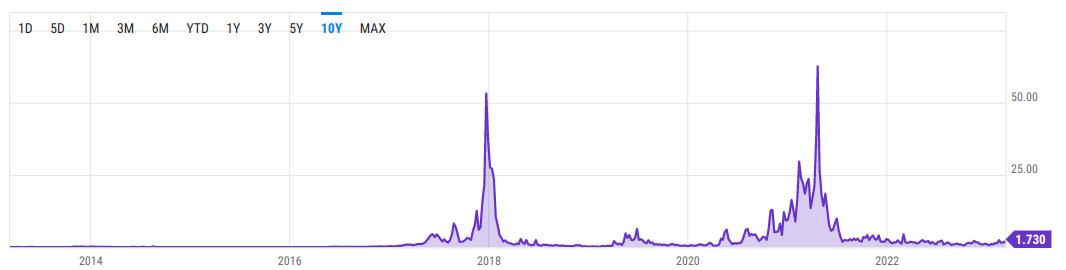
\includegraphics[scale=0.3]{imgs/feerate_blocks.png}
    \end{center}
    \caption{Fee per block in 2021.}
    \label{fig:fee_x_block}
\end{figure}


Overall, the limited number of transactions and the scalability issues on the Bitcoin network
are significant challenges that need to be addressed in order that the network continues
to grow and evolve. There are various proposals, such as \emph{Side Chain} and \emph{Lightning Network}, 
and the Lightning Network is deeply discussed inside Section \ref{sec:lightning_network}.


\section{Bitcoin Transactions}

Transactions are a fundamental part of Bitcoin. In fact, the entire system is designed to ensure
the creation, propagation, and publication of transactions on the blockchain, but these
transactions are conceptually different from the transactions we are used to.
For example, a transaction in a relational database represents an event that triggers a
change in the state within the database, where, in case of malfunctions, the database returns
to the previous condition before the event was triggered.
% FIXME how this transaction are conceptually different? in this case the bitcoin 
% blockchain is atomic
The transactions of Bitcoin are conceptually different.

The transactions are generated by a wallet and propagated to the network
where there are special nodes called \emph{miners} that collect the transactions,
validate them, and build a new block that will be proposed to be stored inside 
the blockchain. During this process, the miners perform the proof of work as 
described in \cite{Palazzo_Estrazione_di_Informazioni_2021}.
Another interesting aspect of Bitcoin transactions is the concept of 
Unspent Transactions Output (UTXOs), as described in \cite{nakamoto2009bitcoin},
and the mechanism to spend a transaction.
A transaction is a data structure (as shown in Table \ref{tab:rawtxbitcoinc}) that contains the core information
of Bitcoin transaction: 

\begin{table}[H]
    \centering\small
       \begin{tabular}{|c|c|}
        \hline
        \multicolumn{2}{|c|}{\textbf{RawTransaction}} \\
        \hline
        \multicolumn{1}{|c|}{Type} & \multicolumn{1}{c|}{Name} \\       
        \hline \hline
        $int32\_t$ & version   \\
        \hline
        $uint8\_t$ & marker \\
        \hline
        $uint8\_t$ & flag \\
        \hline
        CompactSize & numberTxIn \\
        \hline
        vector<TransactionInput> & transactionsInput \\
        \hline
        CompactSize & numberTxOut \\
        \hline
        vector<TransactionOutput> & transactionsOutput \\
        \hline
        vector<TransactionWitness> & transactionsWitness \\
        \hline
    \end{tabular}   
    \caption{Transaction struct \cite{Palazzo_Estrazione_di_Informazioni_2021}.\label{tab:rawtxbitcoinc}}
\end{table}

\begin{itemize}
    \item {\bf RawTransaction}: Main transaction concept that contains the information
        regarding the transactions input and the output of the transaction;
    \item {\bf transactionsOutput}: A wallet, while creating a transaction, will spend some previous
        transaction output (input transaction) and generate a new transaction called \emph{output transaction}.
    \item {\bf transactionsInput}: A transaction spends a previous transaction output contained
        inside UTXOs set, and this kind of transaction is included inside
        the transaction input array;
    \end{itemize}


\begin{example}\label{ex:how_spend_bitcoin}
    Alice wants to pay Bob with bitcoin, so in order to do that Alice
    uses her own UTXO to pay Bob. The wallet of Alice, in this case, creates a new transaction
    capable of \emph{unlocking} the Alice UTXO. At the same time, the wallet creates 
    a new transaction output that Bob owns (that only Bob can unlock) by including it inside the transactions output array. 

    In this way, Alice consumed the UTXO, which means she spends bitcoins and Bob receives bitcoins by collecting UTXO that he owns. 
    If Bob wants to pay Sara, he should repeat the previous step and create a transaction output that Sara can own. This overall process described in this example is depicted in  Figure \ref{fig:lockunlockexample}.

    {\centering
     \vspace{5pt}
      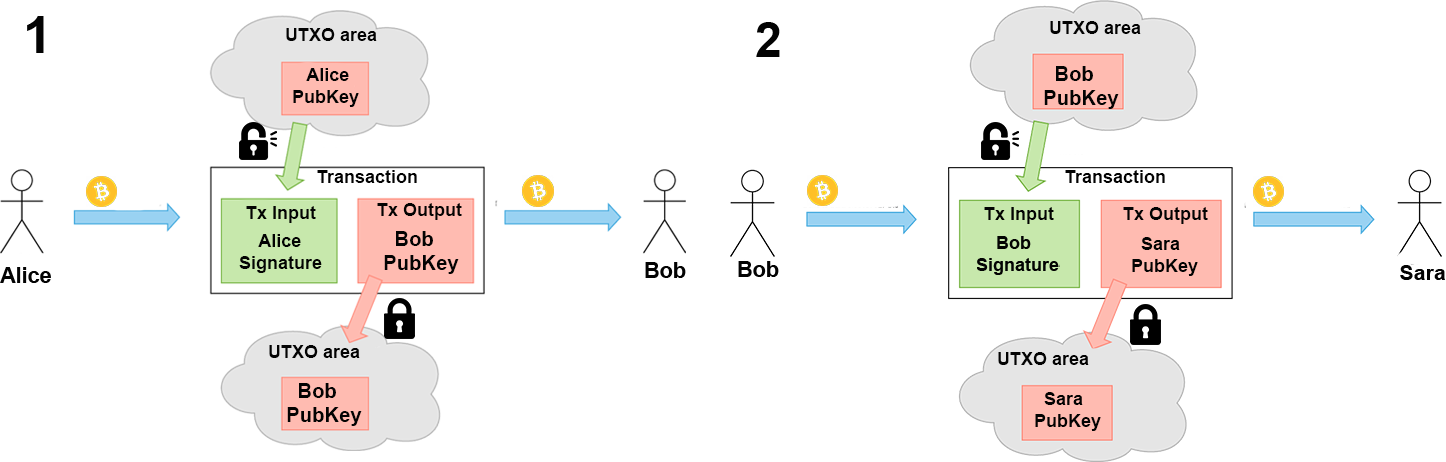
\includegraphics[scale=0.3]{imgs/DiagramUnlocLockUTXO.png}
      \captionof{figure}{UTXO usage as described inside the example \cite{Palazzo_Estrazione_di_Informazioni_2021}.\label{fig:lockunlockexample}}
      \vspace{10pt}
     \par}
\end{example}

%In this section, there is only a general discussion about the transactions, and it is not taken into count
%what happens if the UTXO is not consumed in total! In the paper \cite{Palazzo_Estrazione_di_Informazioni_2021}
%there is a deep discussion on how Bitcoin Transactions work.

We provided here only a very general and high-level discussion about transactions. For a deeper discussion, we refer the reader to \cite{Palazzo_Estrazione_di_Informazioni_2021}.

\section{Bitcoin Script}

In order to implement the transaction verification, there is a need to have
a kind of identification system, and in Bitcoin this system is implemented by a private and public key.
In Example \ref{ex:how_spend_bitcoin}, we showed  that Alice, in order to pay Bob, needs to 
own a transaction, and in other to spend this transaction that Alice owns, the wallet should
create a new transaction capable of unlocking the previous one. 

In this section, we define what ``\emph{owns} a transaction'' means, and how it is possible
to unlock this type of transaction with a new one. 

\subsection{Bitcoin Script Basics}

The input and output transaction described inside Table \ref{tab:rawtxbitcoinc} are 
implemented with a different struct as described inside  Table \ref{tab:tx_in_and_out}.

\begin{table}[ht]
    \centering
    \begin{tabular}{p{5cm}p{5cm}}
        \begin{tabular}{|c|c|}
            \hline
            \multicolumn{2}{|c|}{\textbf{TransactionInput}} \\
            \hline \hline
            \multicolumn{1}{|c|}{Type} & \multicolumn{1}{c|}{Name} \\
            \hline
            Outpoint & outpoint   \\
            \hline
            CScript & scriptSig \\
            \hline
            $uint32\_t$ & nSequence \\
            \hline
        \end{tabular}
         &
         \begin{tabular}{|c|c|}
             \hline
             \multicolumn{2}{|c|}{\textbf{TransactionOutput}} \\
             \hline \hline
             \multicolumn{1}{|c|}{Type} & \multicolumn{1}{c|}{Name} \\
             \hline
             $int64\_t$ & nValue   \\
             \hline
             CScript & scriptPubKey \\
             \hline
         \end{tabular}
    \end{tabular}
    \caption{Input and output transaction struct of Bitcoin Code \cite{Palazzo_Estrazione_di_Informazioni_2021}.}
    \label{tab:tx_in_and_out}
\end{table} 

The most important type for this section is the \emph{CScript} type, which stores the information
of the transaction owners. In particular, inside the input transaction, the 
input contains a condition that is able to unlock (verify) a previously created  
output transaction (UTXO), and the CScript inside the output
transaction contains the condition that needs to be verified in order to unlock
the transaction. The last case is also known as \emph{spending condition}.
% TODO: what is the spending condition
The condition is specified with a stack-based language called \emph{Bitcoin Script}. 
This language is not \emph{Turing Complete}, and this means that it is 
not possible to express complex operations or execute stateful programs, as described 
in \cite{Palazzo_Estrazione_di_Informazioni_2021}.

The execution of a transaction has two possible results, that is: 

\begin{itemize}
    \item {\bf True}: The unlocking script has succeeded in fulfilling the 
        conditions imposed by the lock script, 
        and therefore the input is a valid authorization to spend UTXO;
    \item {\bf False}: If some of the script conditions are not verified.
\end{itemize}

\begin{example}\label{ex:p2ms_example}
    An example of a Bitcoin Script program is called \emph{pay-to-multisignature} (P2MS)
    that defines an M:N (many-to-many) condition where M is the minimum number of signatures required 
    to verify the lock script and N is the total number of public keys. 

    The code in Listing \ref{code:p2ms} shows a full example of a script:

    \begin{lstlisting}[language=bitcoinscript, caption={Full example of pay-to-multisignature script.}, label={code:p2ms}]
    OP_0 <A Signature> <B Signature>
    OP_2 <Public key A> <Public key B> <Public key C> OP_3 OP_CHECKMULTISIG
    \end{lstlisting}

    OP\_0 acts as a placeholder for a bug in the implementation of OP\_CHECKMULTISIG, 
    whose sole purpose is to work around a bug that has accidentally become a consensus rule. The stack 
    will initially be populated with the values from the unlock script.
    In this case, the presence of the OP\_0 operator implies that the stack is empty when encountered, and 
    a stack state is shown in Figure \ref{fig:stackmultsing01}.

    {\centering
    \vspace{15pt}
    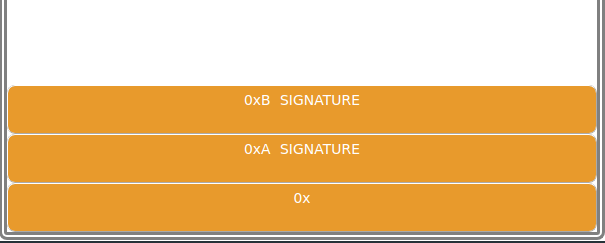
\includegraphics[scale=0.35]{imgs/script/multisig/1.png}
    \captionof{figure}{Stack state after the execution of the lock script (scriptSig) in the stack.\label{fig:stackmultsing01}}
    \vspace{10pt}
    \par}

    The OP\_2 operator checks that there are 2 elements in the stack, then the three 
    public keys are pushed onto the stack, resulting in a state as shown in Figure \ref{fig:stackmultsing02}

    {\centering
    \vspace{15pt}
    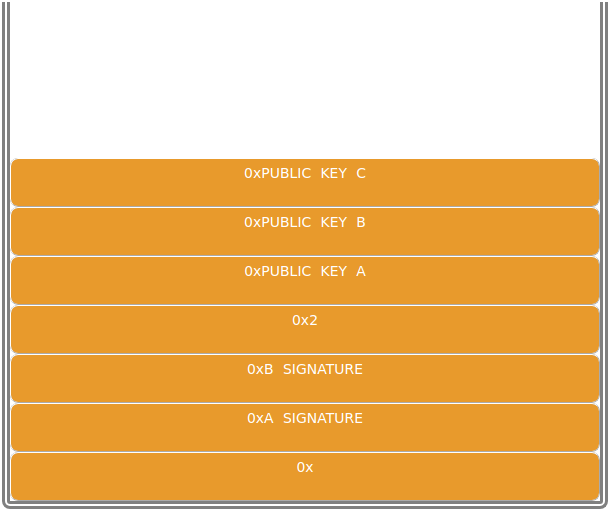
\includegraphics[scale=0.35]{imgs/script/multisig/2.png}
    \captionof{figure}{Stack state after the the check with the OP\_2 operator.\label{fig:stackmultsing02}}
    \vspace{10pt}
    \par}
   
    Finally, the signatures are verified against the public keys using the 
    OP\_CHECKMULTISIG operator iteratively, meaning that  the first signature is compared to 
    all the public keys and this action is repeated for all signatures pushed onto the stack, 
    as shown in Figure \ref{fig:stackmultsing03}.
 
    {\centering
    \vspace{15pt}
    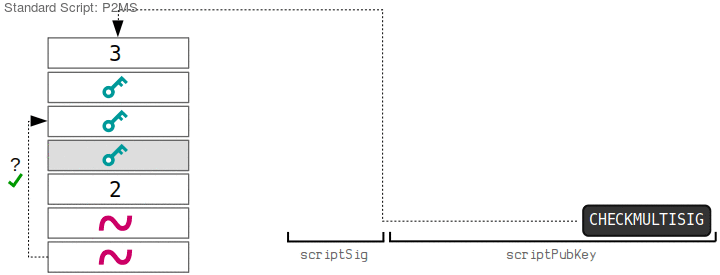
\includegraphics[scale=0.30]{imgs/script/multisig/3.png}
    \captionof{figure}{OP\_CHECKMULTISIG example that verify the keys \cite{learnmeabitcoin:p2ms}.\label{fig:stackmultsing03}}
    \vspace{10pt}
    \par}

\end{example}

In conclusion, the example \ref{ex:p2ms_example} shows that Bitcoin script is a simple
language, but with time that language has arrived at a level where it is possible to
express smart contract that allows the development of new technology on top of Bitcoin as \emph{base layer},
and in the code in Listing \ref{code:htlc_example} it shows a Hash Time Lock contract used in the Lightning Network 
and deeply discussed in \ref{sec:htlc_intro}.


\begin{lstlisting}[language=bitcoinscript, caption={Hash Time Lock contract first example.}, label={code:htlc_example}]
OP_IF
    # Penalty transaction
    <revocationpubkey>
OP_ELSE
    `to_self_delay`
    OP_CHECKSEQUENCEVERIFY
    OP_DROP
    <local_delayedpubkey>
OP_ENDIF
OP_CHECKSIG
\end{lstlisting}



